\section{Redes  \glsentryshort{sdn}}
\label{sec:sdn}


El paradigma \gls{sdn} \cite{nadeau2013sdn} se refiere a una arquitectura de red en la que se separa el plano de control de la red para centralizarlo en un controlador único. Esta estructura permite lograr una administración de red más centralizada y flexible \cite{nadeau2013sdn}. La idea del \gls{sdn} comenzó a gestarse en la Universidad de Stanford en 2003, cuando el profesor asociado de ese entonces, Nick McKeown, planteó las limitaciones de las redes convencionales y la necesidad de replantear cómo operaban los \textit{backbones} \cite{sdnBegins}. En 2011, se acuñó el término \gls{sdn}, al mismo tiempo que se lanzó la organización \gls{onf} \cite{onf}, encargada de establecer estándares y promover la difusión del \gls{sdn}.

\subsection{Arquitectura del paradigma \glsentryshort{sdn}}

La arquitectura \gls{sdn} se destaca por su dinamismo, rentabilidad y adaptabilidad, lo que la convierte en una solución ideal para las demandas actuales de las redes de comunicaciones. Como se ha mencionado anteriormente, esta arquitectura se basa en la separación del plano de control y el plano de datos, trasladando el control a una entidad central llamada controlador. A través de esta entidad, se ofrecen interfaces que permiten a las aplicaciones de servicios de red utilizarlas. Esto hace que el control de la red sea programable directamente, lo que agiliza y dinamiza su gestión.\\
\\
La arquitectura \gls{sdn} se divide en tres capas, como se muestra en la figura \ref{fig:sdnBasicArch}. La primera capa es el plano de datos, donde se encuentran todos los elementos de red responsables del reenvío de los datos. La segunda capa es el plano de control, compuesto por diferentes controladores \gls{sdn}. Por último, la capa de aplicación alberga todas las aplicaciones que se comunican con el controlador \gls{sdn}.\\
\\
Estas capas se comunican entre sí a través de interfaces abiertas. Por ejemplo, la interfaz \textit{Southbound} permite programar el estado de reenvío de los elementos de red en el plano de datos. Por otro lado, la interfaz \textit{Northbound} permite la comunicación entre las aplicaciones y los controladores \gls{sdn}, permitiendo la obtención de datos y el ajuste de parámetros mediante una API-Rest. Además, existen otras interfaces, como \textit{Westbound} y \textit{Eastbound}, que se han consolidado en los últimos años para interconectar controladores y establecer políticas comunes entre diferentes dominios \gls{sdn}.\\

% Foto 
\begin{figure}[ht]
    \centering
    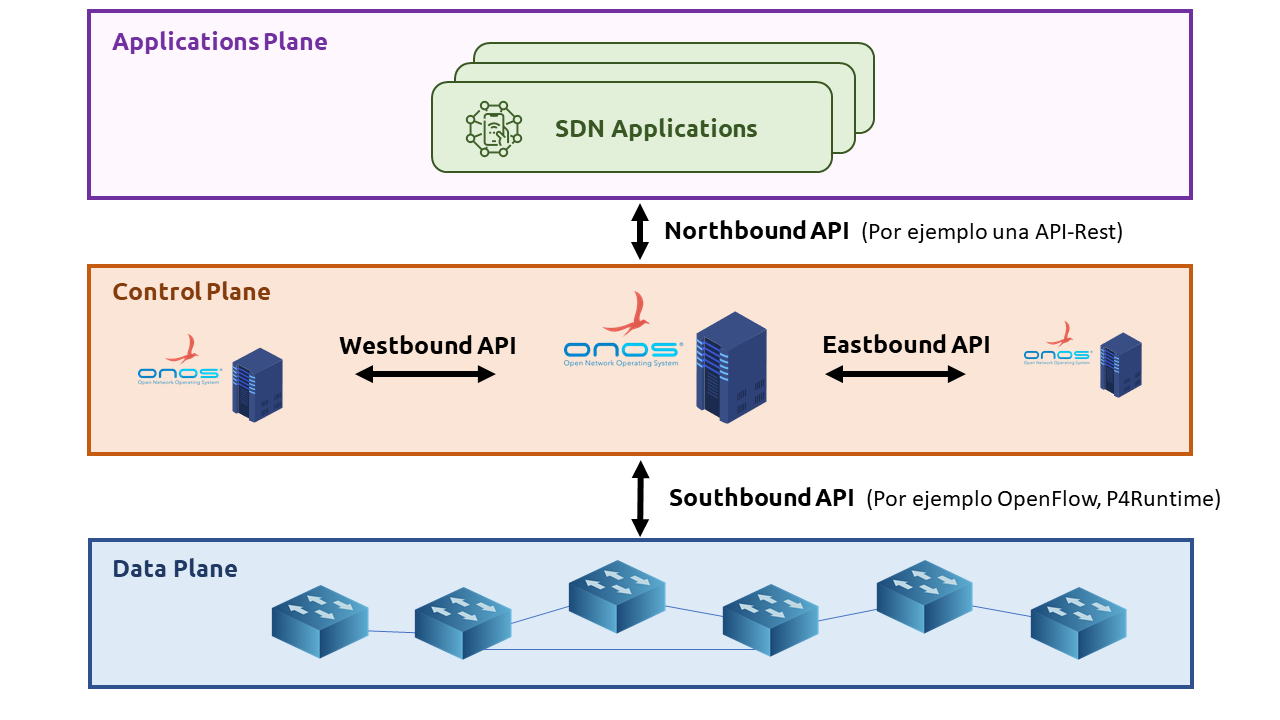
\includegraphics[width=0.9\textwidth]{archivos/img/teoria/sdn_arch.png}
    \caption{Arquitectura típica \glsentryshort{sdn} \cite{carrascal2020diseno}}
    \label{fig:sdnBasicArch}
\end{figure}


\subsection{Protocolo OpenFlow}

Existen varios protocolos para el control de los elementos de red desde el controlador, pero el más ampliamente utilizado es OpenFlow. OpenFlow es un protocolo de la interfaz \textit{Southbound} que establece la comunicación entre los controladores \gls{sdn} y los elementos de red para configurar el plano de forwarding de estos últimos. La especificación de este protocolo está definida por la \gls{onf}\footnote{\url{https://www.opennetworking.org/software-defined-standards/specifications/}}, y cuenta con varias versiones, siendo la más reciente la versión \texttt{1.5.1} lanzada en 2015.\\
\\
El concepto fundamental en OpenFlow es el flujo (\textit{flow}), el cual está compuesto por paquetes que se han clasificado según reglas específicas. Estas reglas se encuentran en las tablas de flujo (\textit{flow table}) y suelen estar relacionadas con los puertos de entrada o los valores de los campos de cabecera del paquete. Cuando los criterios de una regla coinciden con los valores de un paquete entrante, se produce una coincidencia (\textbf{\textit{match}}).\\
\\
Cuando se produce una coincidencia (\textit{match}), el paquete se somete a una serie de instrucciones asociadas a la regla con la que ha coincidido. Estas instrucciones pueden incluir la medición del paquete, la aplicación de acciones específicas o el enrutamiento hacia otra tabla de flujo. De esta manera, al completar las tablas de flujo con reglas suministradas por el controlador \gls{sdn}, se configura el estado de reenvío del switch en cuestión \cite{nadeau2013sdn}. A continuación, en la figura \ref{fig:openflow_arch}, se puede apreciar los elementos básicos que suele contener un switch Openflow. Más adelante en la sección \ref{subsec:BOFUSS} sobre \textit{software switches} se estudiarán en profundidad los elementos básicos que componen un agente \gls{sdn} que implementa un agente Openflow.


\begin{figure}[ht]
    \centering
    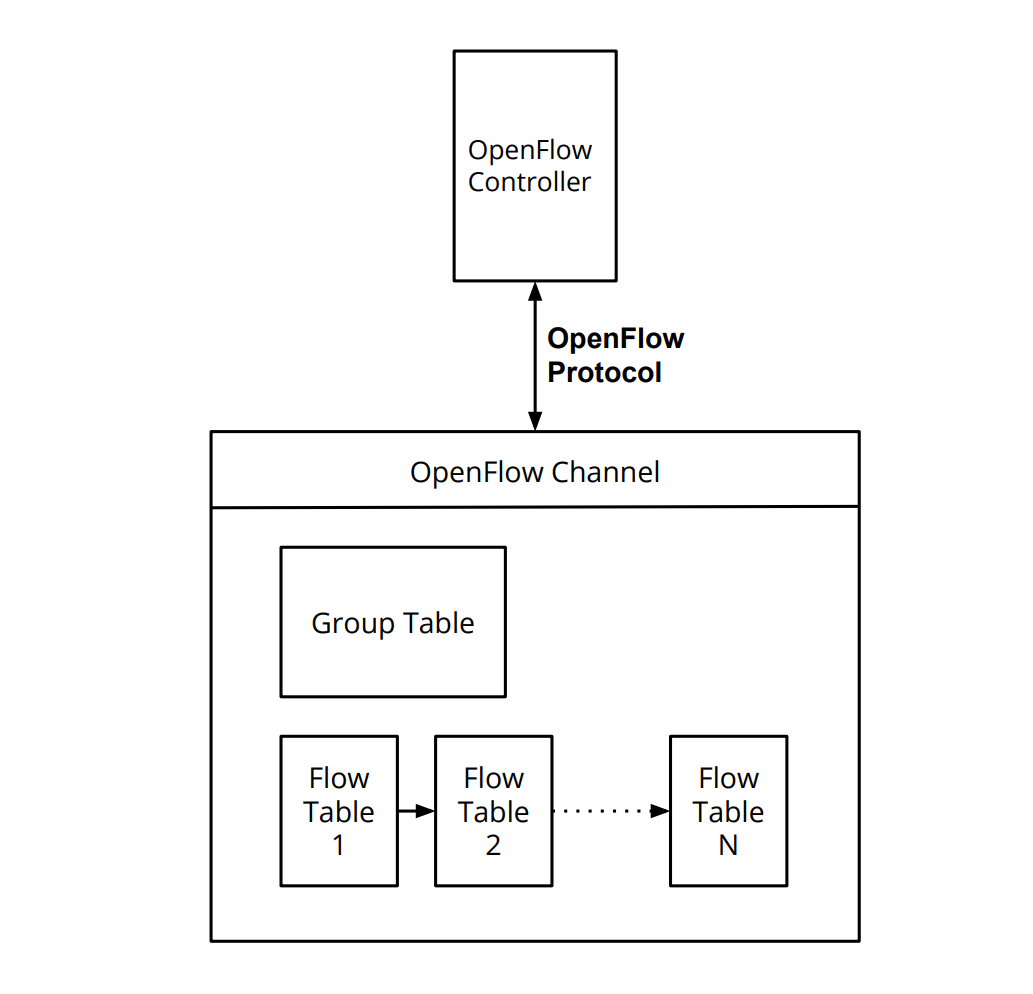
\includegraphics[width=0.6\textwidth]{archivos/img/teoria/openflow_arch.png}
    \caption{Arquitectura básica de agente OpenFlow \cite{fernandes2015software}}
    \label{fig:openflow_arch}
\end{figure}
